\documentclass[11pt,a4paper]{article}

\usepackage{../../templates/style}


\begin{document}

\begin{problem}{ขวดน้ำ (crystal)}{standard input}{standard output}{1 second}{32 megabytes}

ณ ค่ายแห่งหนึ่ง ซึ่งจัดโดย\textit{สมาคมสวมแว่นแห่งประเทศไทย(สสวท.)} มีการเก็บขวดน้ำที่ด้านหลังห้องเรียน เพื่อรอการนำไปรีไซเคิลลดโลกร้อน

อยู่มาวันหนึ่ง \textit{"ชายเลย์"} เพื่อนร่วมค่ายของคุณนำขวดน้ำมาตั้งซ้อนกันอย่างแปลกประหลาด โดยการเรียงขวดน้ำของเขามีกฎการเรียงดังนี้

\begin{enumerate}

\item ที่ฐานของกองขวดน้ำประกอบไปด้วยขวดน้ำ $N$ ขวดเรียงชิดติดกัน
\item ขวดน้ำแต่ละขวดต้องตั้งอยู่บนขวดน้ำสองขวดที่อยู่ชั้นด้านล่าง
\item ในชั้นที่ไม่ใช่ชั้นล่างสุด สามารถวางขวดน้ำไม่ติดกันได้
\item ที่ค่ายมีขวดน้ำอยู่เป็นจำนวนมากมายจนถือว่าพอสำหรับการวางแบบใดๆ และขวดน้ำทุกขวดลักษณะเหมือนกันหมด
\end{enumerate}

(ถ้ายังไม่เข้าใจกรุณาดูรูปภาพประกอบข้อมูลนำเข้าที่ 2)
ชายเลย์ต้องการหาวิธีการเรียงขวดน้ำทุกรูปแบบเท่าที่เป็นไปได้เขาจึงวานให้คุณช่วย


\bigskip
\underline{\textbf{โจทย์}}  จงเขียนโปรแกรมรับจำนวนขวดที่ชายเลย์ใช้เป็นฐานของกองขวดน้ำ จากนั้นคำนวณหาจำนวนวิธีการเรียงขวดน้ำทั้งหมดที่เป็นไปได้


\InputFile

\textbf{มีบรรทัดเดียว} รับจำนวนเต็มบวก $N$ $(1 \leq N \leq 1\,000)$ แทนจำนวนขวดที่ชายเลย์ใช้เป็นฐานของกองขวดน้ำ

\OutputFile

\textbf{มีบรรทัดเดียว} แสดงจำนวนวิธีการเรียงขวดน้ำทั้งหมด โดยตอบเป็นเศษที่เหลือจากการหารจำนวนดังกล่าวด้วย $10\,001$

\Examples

\begin{example}
\exmp{3}{5}%
\exmp{4}{14}%
\exmp{13}{2826}%
\end{example}

\Note 

\textbf{รูปภาพประกอบตัวอย่างข้อมูลนำเข้าที่ 2} 

\begin{figure}[!h]
\centering
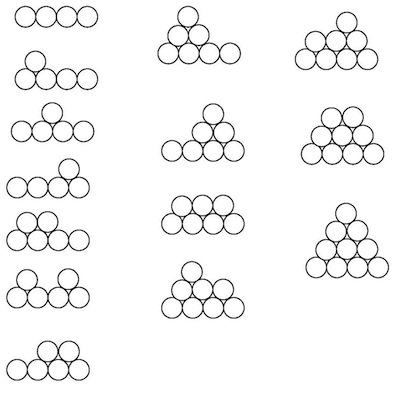
\includegraphics[width=0.5\textwidth]{../latex/img/1172/1172-1.jpeg}
\end{figure}

\begin{itemize}

\item รูปแบบกองขวดน้ำทั้งหมดของชายเลย์ที่มีฐานเป็นขวดน้ำ $4$ ขวด
\item วงกลมแทนขวดน้ำแต่ละขวด
\end{itemize}

\Source

พศิน มนูรังษี

IOI Thailand League 2010 เดือน เมษายน

\end{problem}

\end{document}